\chapter{$H \rightarrow ZZ \rightarrow 4l$}
\justifying
\paragraph{}
The goal of this exercise is to reconstruct the Standard Model (SM) Higgs boson mass, using a selection targeting the four-lepton final state. This is considered a \textit{golden} channel to rediscovered the Higgs because:
\begin{itemize}
    \item there is a \textbf{\underline{ large signal to background ratio}} -- it is easy to discriminate between the peak of the reconstructed four-lepton mass ($m_{4l}$) and the overall flat background shape; 
    \item we have excellent \textbf{\underline{ mass resolution}} -- thanks to the great resolution power of CMS, we have optimal shape reconstruction of $m_{4l}$;
    \item it is a \textbf{\underline{ resolved final state}} -- detection of the four leptons in the final state ensures good discrimination of signal and background.
\end{itemize}

\begin{figure}[!h]
    \centering
    \includegraphics[scale=0.35]{images/plot.png}
    \caption{\justifying{Reconstructed four-lepton invariant mass $m_{4l}$ with 2018 data. The SM Higgs boson signal with $m_H = 125$ GeV, denoted as $H(125)$, and the $ZZ$ backgrounds are normalized to the SM expectation. The $Z+X$ background is normalized to the estimation from data.}}
    \label{higgs_plot}
\end{figure}

\section{Installation \& setup}
\justifying
\begin{tcolorbox}[colback=green!5!white,colframe=green!75!black,width=\textwidth]
Note: ColumnFlown only runs on Linux and may require up to 4 GB of disc space. \tcblower
Also, the machine where you run this exercise must be mounted with CERN AFS.
\end{tcolorbox}

Start by going to the GitLab repository of this exercise:

\texttt{\textcolor{LimeGreen}{\href{https://gitlab.cern.ch/cms-analysis/analysisexamples/columnflow-demo}{\underline{https://gitlab.cern.ch/cms-analysis/analysisexamples/columnflow-demo}}}}

To have your own copy of the code, fork the repository into your personal area. You can do this by clicking the \code{Fork} button on the upper right corner of the page. To set your Project URL please type your CERN username in the \code{Select a namespace} option.

\begin{figure}[!h]
    \centering
    \includegraphics[scale=0.62]{images/gitlab.png}
\end{figure}
\begin{figure}[!h]
    \centering
    \includegraphics[scale=0.62]{images/fork1.png}
\end{figure}

After clicking the \code{Fork project} button, your fork url should be:

\texttt{https://gitlab.cern.ch/<cern\_username>/columnflow-demo}

\newpage
In your forked project, go to the \code{Code} button on the right hand side of the page and copy the address under the \code{Clone with HTTPS} option. If you have an SSH key registered on GitLab prior to this exercise, you can also use the \code{Clone with SSH} option.

\begin{figure}[!h]
    \centering
    \includegraphics[scale=0.62]{images/fork2.png}
\end{figure}

Next, open a new terminal window and clone your code to your machine by running \underline{one of} the following commands (depending on which cloning method you chose):

\begin{lstlisting}[language=bash]
git clone --recursive https://gitlab.cern.ch/<cern_username>/columnflow-demo.git
\end{lstlisting}
\begin{lstlisting}[language=bash]
git clone --recursive ssh://git@gitlab.cern.ch:7999/<cern_username>/columnflow-demo.git
\end{lstlisting}

The directory you have thus created will be referred to as \code{basedir}. You can now go inside your local repository and install ColumnFlow. The \code{setup.sh} bash script will initialize the software environment with \code{micromamba}. Here, we define \code{dev} as the setup name, but you are free to name it as you wish.

\begin{lstlisting}[language=bash]
cd columnflow-demo
source setup.sh dev
\end{lstlisting}

You will be asked to define a series of variables, the first of which is your CERN username. For all other variables you can keep the default value by just pressing \code{Enter}. Variables specific to this exercise will start with \code{H4L\_}, while ColumnFlow specific variables start with \code{CF\_}. You can find all variables in the \code{.setups/dev.sh} bash file. We invite you to check out this file and familiarize yourself with these variables.

\begin{figure}[!h]
    \centering
    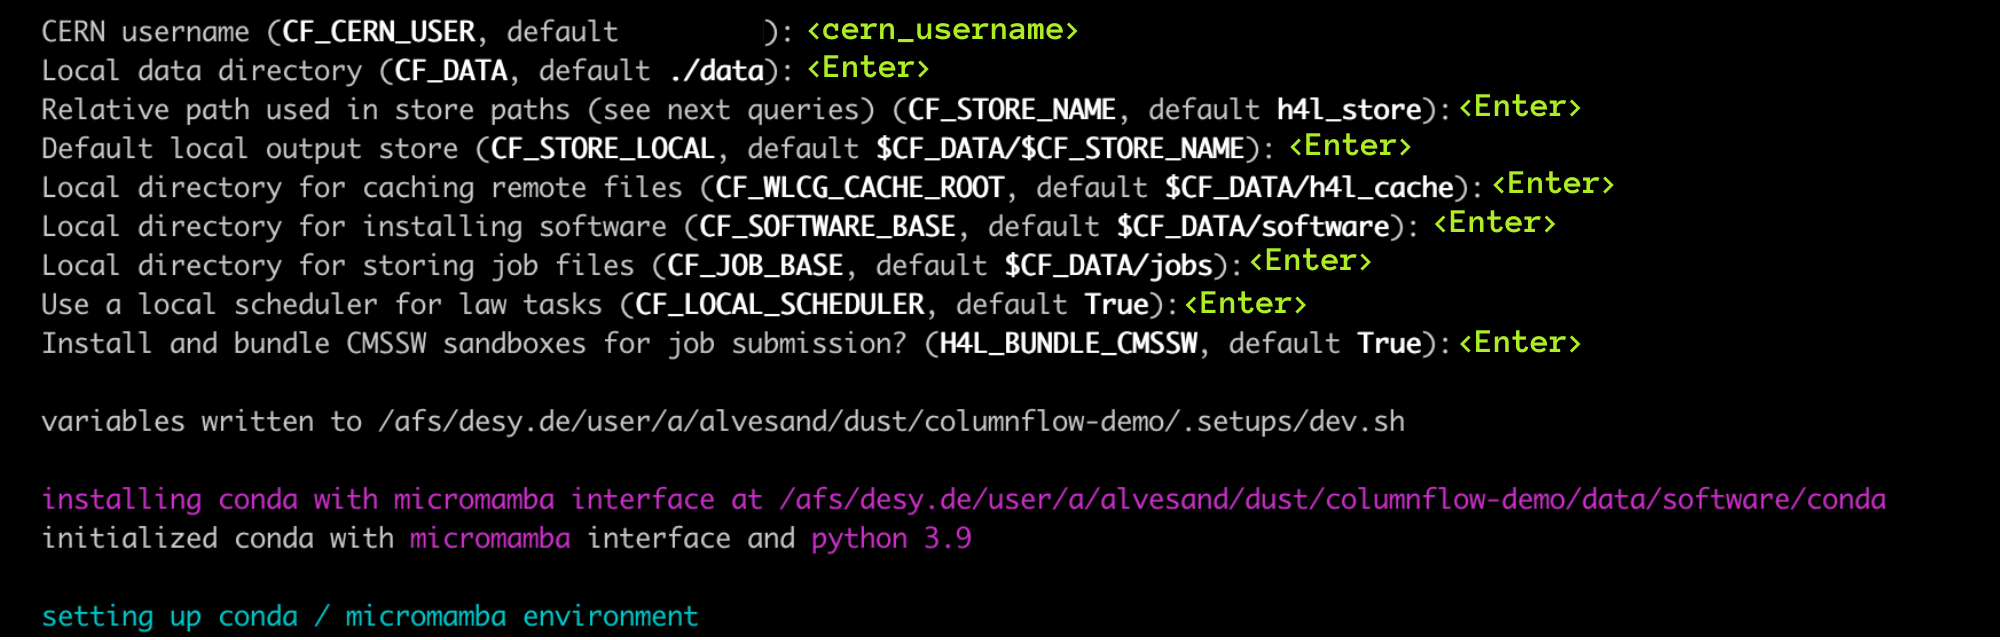
\includegraphics[scale=0.62]{images/setup.png}
\end{figure}

Note that the first installation of the software can take \underline{up to several minutes}.

Every time you want to work with ColumnFlow (e.g.\ if you open a new terminal window), you will need to source the \code{setup.sh} script again.

Once the installation is complete you should see a line of green text stating that the analysis has been successfully set up. You are now ready to start working with ColumnFlow!

\begin{figure}[!h]
    \centering
    \includegraphics[scale=0.62]{images/setup2.png}
\end{figure}

Inside of your newly created \code{columnflow-demo} directory, you will find the following project structure:
\begin{figure}[!h]
    \centering
    \includegraphics[scale=0.62]{images/CF_demo.png}
\end{figure}

%\subsection{ColumnFlow Tasks}

This exercise is organized in the form of \code{law} tasks, where different tasks create some form of output. You can view the available tasks by running:
\begin{lstlisting}[language=bash]
law index --verbose
\end{lstlisting}

This exercise will focus on the following tasks:

\begin{itemize}
    \item \texttt{\textcolor{LimeGreen}{cf.CalibrateEvents}} / \texttt{\textcolor{LimeGreen}{cf.SelectEvents}}
    \item \texttt{\textcolor{LimeGreen}{cf.ProduceColumns}}
    \item \texttt{\textcolor{LimeGreen}{cf.PlotCutflow}}
    \item \texttt{\textcolor{LimeGreen}{cf.PlotVariables1D}} / \texttt{\textcolor{LimeGreen}{cf.PlotVariables2D}}
    \item \texttt{\textcolor{LimeGreen}{cf.CreateDatacards}}
\end{itemize}

By default, these tasks will save their output on a remote file system (e.g.\ \texttt{WLGC}), for which you will require a \code{voms-proxy}. If you would like to save certain/all outputs locally, we recommend to create a directory on a system with a larger amount of disk space (e.g.\ \texttt{EOS}). For such cases, you will need to update the \code{law.cfg} file accordingly.


\section{Analysis strategy}

In order to find Higgs boson candidates, we need to reconstruct the four leptons in the final state. To select the four lepton candidates in the first place, we will need to write a \CCSPStlye{Selector} (Section~\ref{sec:selector}).

%, which will filter out all physics objects that do not fulfill the selection criteria. In this selector, we will implement \underline{kinematic cuts}, \underline{vertex cuts} and \underline{Isolation \& ID} criteria. We will also implement \underline{trigger selections} such that only events interesting for the $ZZ$ analysis are selected.

\begin{figure}[!h]
    \centering
    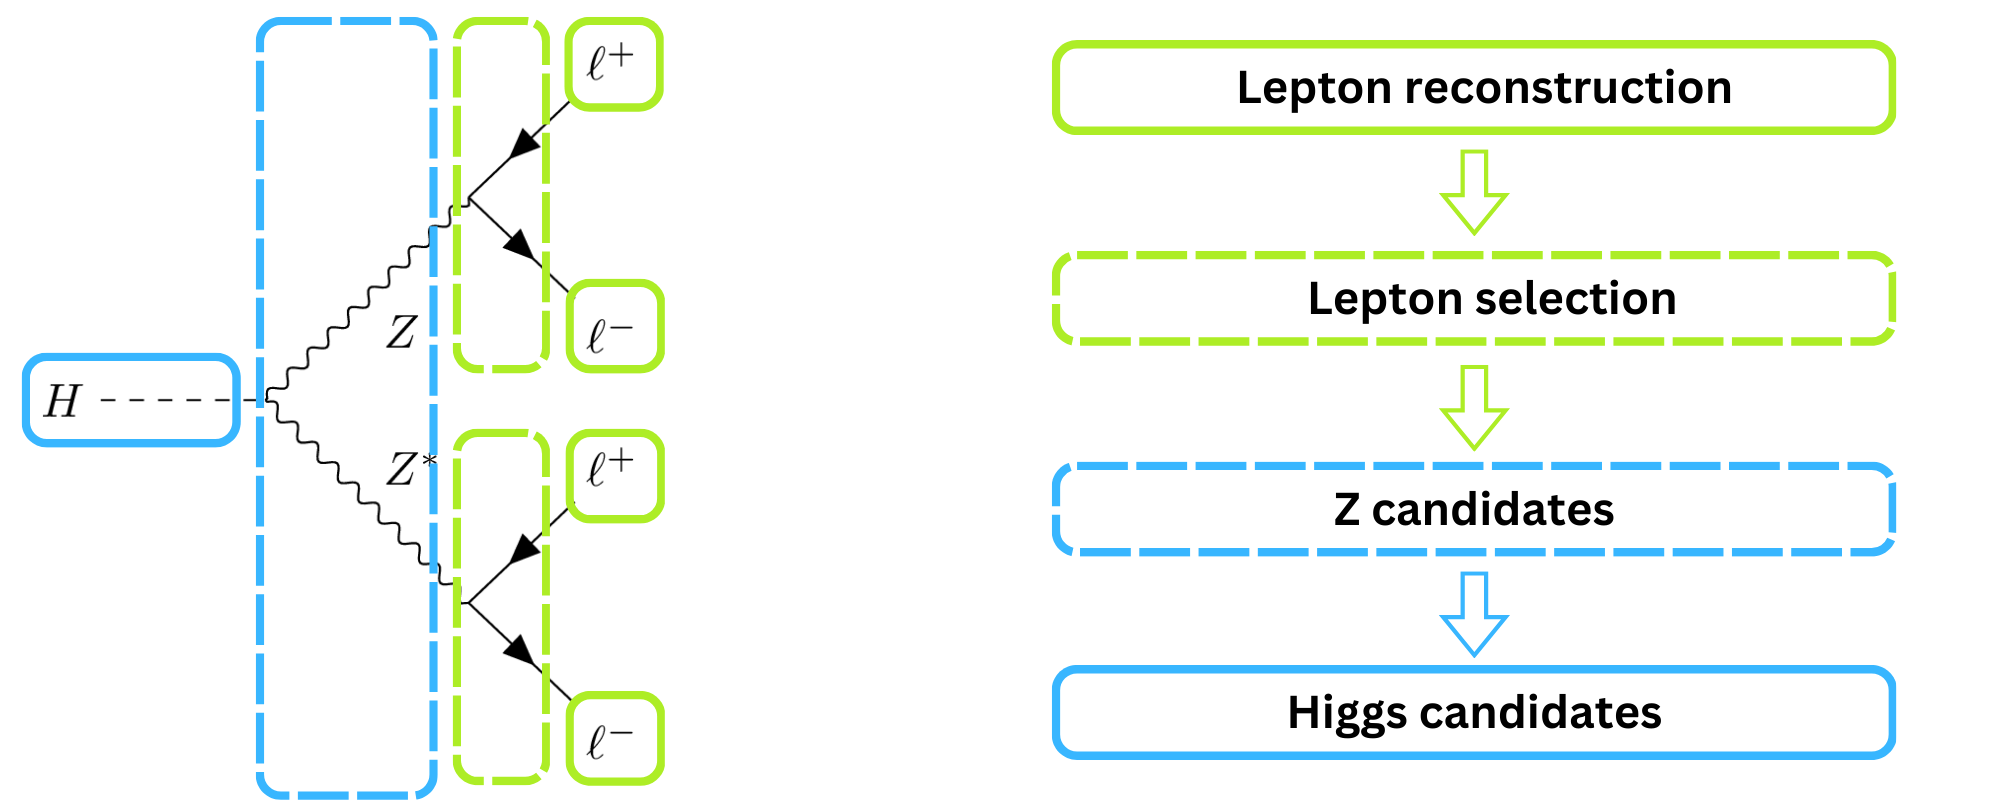
\includegraphics[scale=0.62]{images/strategy.png}
\end{figure}

\section{Writing a Calibrator}\label{sec:calibrator}
\section{Writing a Selector}\label{sec:selector}

The \CCSPStlye{Selector} class should be used to implement analysis selections.
This is a crucial step in the workflow since the decision to keep or reject objects or even whole events is performed here.
Since the selection usually depends on for example four-momenta of the objects within the events, it is executed after the calibration.
The corresponding task is called \CCSPStlye{cf.SelectEvents}.

For more information, please consider Ref.~\cite{cf_repo}.

\renewcommand{\arraystretch}{1.5}
\begin{table}[h!]
    \centering
    \begin{tabular}{|m{4cm}|m{5cm}|m{5.5cm}|}
    \hline
    & \textbf{Electrons} & \textbf{Muons} \\ \hline
    \textbf{Kinematic cuts} &
    \begin{itemize}[leftmargin=*]
    \item $p_T^e > 7$ GeV
    \item $|\eta^e| < 2.5$
    \end{itemize} &
    \begin{itemize}[leftmargin=*]
        \item $p_T^\mu > 5$ GeV
        \item $|\eta^\mu| < 2.5$
    \end{itemize} \\ \hline
    \textbf{Vertex cuts} &
    \begin{itemize}[leftmargin=*]
        \item $d_{xy} < 0.5$
        \item $d_z < 1$ cm
        \item $SIP < 4$
    \end{itemize} &
    \begin{itemize}[leftmargin=*]
        \item $d_{xy} < 0.5$
        \item $d_z < 1$ cm
        \item $SIP < 4$
    \end{itemize} \\ \hline
    \textbf{Isolation \& ID for \newline 'tight' working point} & Dedicated BDT targeting \newline prompt electrons. & Select only muons within \newline a well-defined cone ($R=0.35$). \\ \hline
    \end{tabular}
    \Caption{Selection criteria for leptons.}{Shown are the selection cuts for electrons/muons at the 'loose' working point, with the last row defining the extra requirement for the leptons to pass the 'tight' working point.}
    \label{leptonSelection}
\end{table}

In this part of the tutorial, we will write selections for electrons and muons.
In the script \code{h4l/selection/lepton.py} you can find the base structure to implement two \CCSPStlye{Selector} modules, \code{electron\_selection} and \code{muon\_selection}.
Each of these objects uses the relevant event information for its implementation.


\textbf{\underline{Electron Selection}}

For \code{electron\_selection}, the electron kinematic information is first loaded into the \code{uses} set.
Then, information that is dependent on the nanoAOD version is loaded. In this case, which MVA (Multi-Variate Analysis) flag should be used.
Notice that we use the union operator \code{|} to append either \code{Electron.mvaFall17V2Iso} or \code{Electron.mvaHZZIso} to the set containing the kinematic variables.
Lastly, to perform four-vector calculations, we also recquire \code{attach\_coffea\_behavior}, which is imported at the beginning of the script from \code{columnflow.selection.util}.


This \CCSPStlye{Selector} object also has two more dependencies, \code{exposed} and \code{sandbox}.
The first one determines whether or not the \CCSPStlye{Selector} object is available from the command line.
As mentioned in the last section, \code{sandbox} specifies the software enviorment where this \CCSPStlye{Selector} will be executed.

\newpage
\begin{itemize}
    \item {
        \textbf{\underline{Loose Electrons}} -- Within the main body of \code{electron\_selection}, all selections should be applied.
        Note that the minimum transverse momentum has already been specified in \code{min\_pt}.
        The actual value, in GeV, is set in \code{h4l/config/config\_h4l.py}, and depends on the argument \code{working\_point}.
        In the config file, a dictionary stores two possible values, $15$ for a \code{'tight'} working point (default value), and $7$ for a \code{'loose'} working point.
        Both the transverse momentum and the pseudorapidity selection criteria have already been applied in \code{default\_mask}.
        You should now complete the mask with the remaining selection criteria from Table \ref{leptonSelection}.
    }
    \item {
        \textbf{\underline{Tight Electrons}} -- Finally, you should also add a condition that applies the identification criteria for when \code{working\_point} is set to \code{'tight'}.
        Both the fSCeta and BDT values are set in the function \code{return\_electron\_id\_cuts}, which can be found in \code{h4l/selection/util.py}.
    }
\end{itemize}

After all selections have been applied, the final part of the module sorts all events by their momentum and applies the \code{default\_mask}.
The indices of selected events are then stored in \code{selected\_electron\_idx}.
The \code{electron\_selection} module finally returns both all events and a \CCSPStlye{SelectionResult} class instance.
We initiate the \CCSPStlye{SelectionResult} instance by setting the \code{objects} and \code{aux} (i.e. auxiliary) arguments.
Within \code{objects}, a nested dictionary saves \code{selected\_electron\_idx} as a value to an \code{Electron} key.
The selection mask itself, \code{default\_mask} is stored in \code{aux}.

\begin{exercise}{Writing a Selector -- Electron Selection}[h4l/selection/lepton\_solution.py]
	Refering to Table \ref{leptonSelection}, fill in the missing information in the \CCSPStlye{Selector} module \code{electron\_selection} defined in \code{h4l/selection/lepton.py}.
\end{exercise}

\vspace{0.8cm}

\textbf{\underline{Muon Selection}}

The \code{muon\_selection} module behaves very similarly. In this case, a dedicated software environment is not required.
There is also no information dependent on the nanoAOD version.
Besides the kinematic information, the \code{uses} set also loads muon quality criteria (e.g. if it is a global or tracker muon), identification and isolation information.

\begin{itemize}
    \item {
        \textbf{\underline{Loose Muons}} -- Within the main body of \code{muon\_selection}, a selection mask is now defined \code{selected\_muon\_mask}.
        Similarly to the electron selection, the minimum transverse momentum and pseudorapidity are already defined.
        You should now expand this mask such that:
        \begin{enumerate}
            \item you recquire either a global or tracker muon (for tracker muons \code{nStations} should be a positive);
            \item discard standalone muon if the reconstructed tracks are only present in the muon system (i.e. for standalone muons, you should recquire a positive number of \code{nTrackerLayers});
            \item apply the remaining selection criteria from Table \ref{leptonSelection}.
        \end{enumerate}
    }
    \item {
        \textbf{\underline{Tight Muons}} -- You should now add three conditions to \code{selected\_muon\_mask}:
        \begin{enumerate}
            \item enforce that the low momentum muons ($< 200$ GeV) are ParticleFlow candidates (use the variable \code{isPFcand});
            \item enforce that the high momentum muons ($\geq 200$ GeV) are ParticleFlow candidates OR have a positive \code{highPtId};
            \item use the variable \code{pfRelIso03\_all} to apply the condition in Table \ref{leptonSelection}.
        \end{enumerate}
    }
\end{itemize}

\begin{exercise}{Writing a Selector -- Muon Selection}[h4l/selection/lepton\_solution.py]
	Again refering to Table \ref{leptonSelection}, fill in the missing information in the \CCSPStlye{Selector} module \code{muon\_selection} defined in \code{h4l/selection/lepton.py}.
\end{exercise}

